\documentclass{article}

% General document formatting
\usepackage[margin=2cm]{geometry}
\usepackage[slovak]{babel}
\usepackage[parfill]{parskip}
\usepackage[utf8]{inputenc}
\usepackage{times}
\usepackage{graphicx}
\usepackage{pdflscape}

\begin{document}

\Large
\textbf{Jméno: Patrik Skaloš} \\
\textbf{Login: xskalo01}
\normalsize
\bigskip


\section*{Architektura navrženého obvodu (na úrovni RTL)}
\bigskip

\subsection*{Schéma obvodu}
\bigskip
\begin{figure}[h]
  \begin{center}
    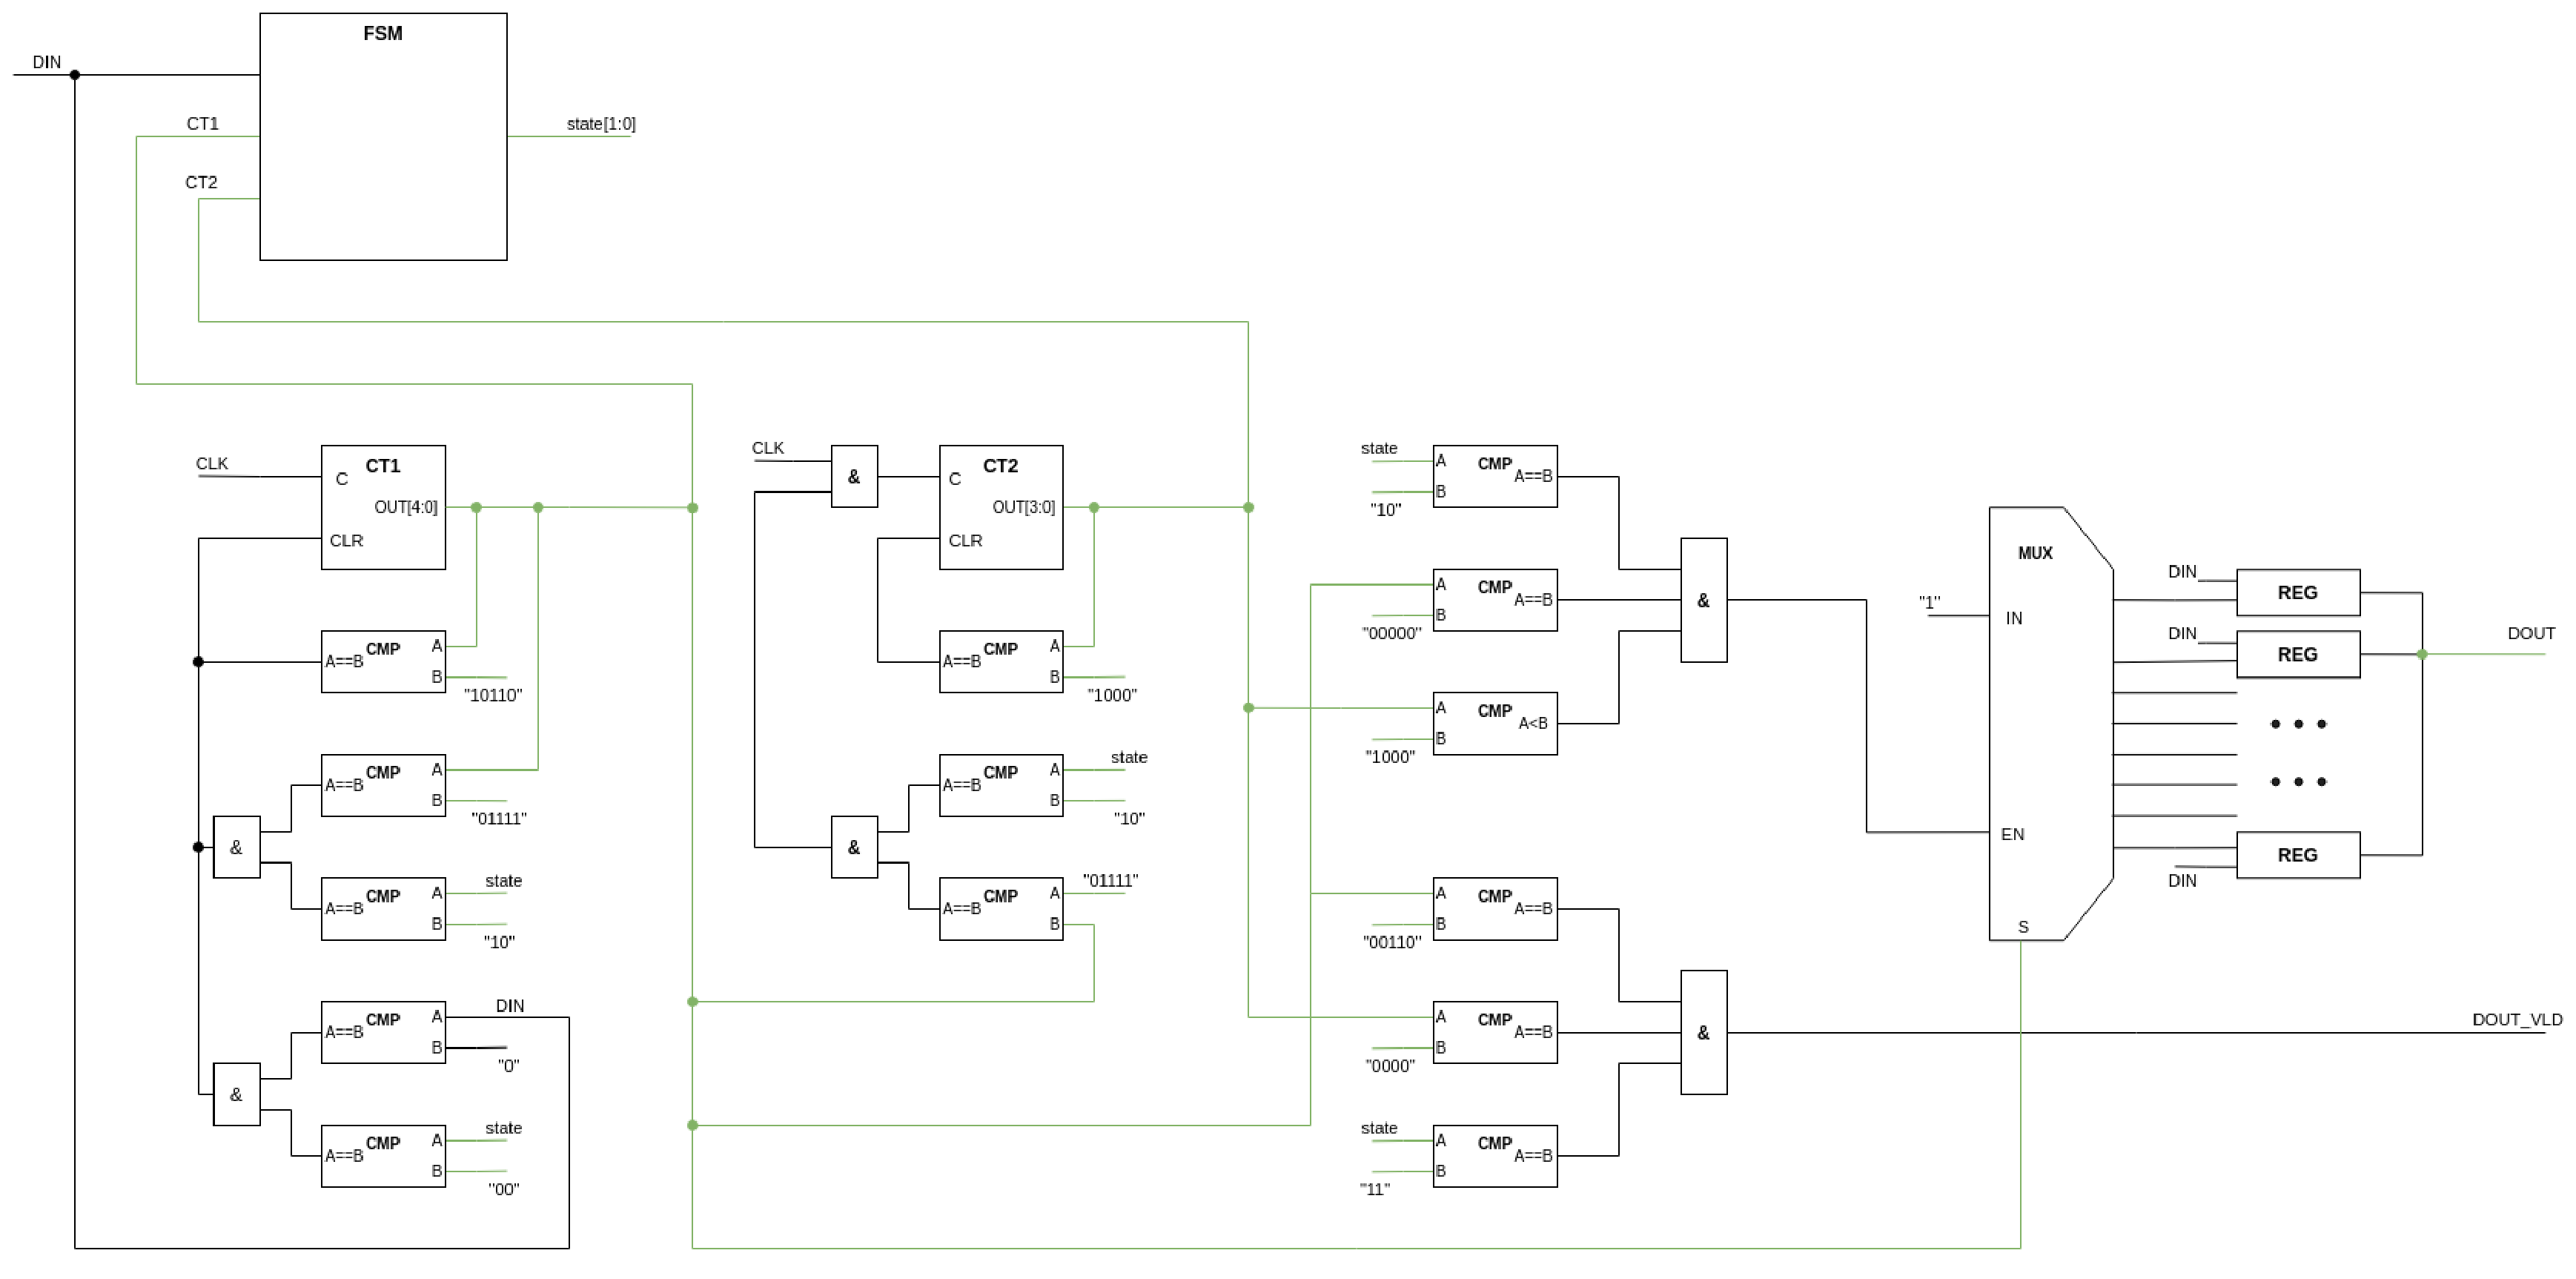
\includegraphics[width=18cm]{src/rtl.eps}
  \end{center}
\end{figure}

\subsection*{Popis funkce}
\bigskip
Obvod je závislý od stavu \textbf{FSM} a jeho najdôležitejšími časťami sú dva 
čítače a multiplexor.
\par
Čítač \textbf{CT1} je použitý na čakanie medzi rôznymi akciami (napríklad
medzi prijímom start bitu a prijímom prvého bitu zaručuje čakanie po dobu
\textbf{24} CLK cyklov), \textbf{CT2} je použitý na počítanie prijatých bitov 
(keď ich je 8, príjem končí). Čítače sú riadené a resetované komparátormi, tie 
tu však nebudem vysvetľovať.
\par
Nakoniec multiplexor jednoducho zapisuje vstupy do registrov, ktorých výstupy 
tvoria \textbf{DOUT} (výstup dát).
\par
Posledná dôležitá časť je hradlo \textbf{AND} a tri komparátory, ktoré 
nastavujú \textbf{DOUT\_VLD} na \emph{log. 1} v prípade, že \textbf{FSM} je v 
stave \uv{finishing} (všetky bity boli prijaté), čítač \textbf{CT1} je na 
hodnote \textbf{6} a \textbf{CT2} na hodnote \textbf{0}. To má za následok 
nastavenie \textbf{DOUT\_VLD} na \emph{log. 1} práve počas posledného CLK cyklu 
stop bitu.

\newpage


\section*{Návrh automatu (Finite State Machine)}
\bigskip

\subsection*{Schéma automatu}
\bigskip
\textbf{Legenda:}
\begin{itemize}
  \item Stavy automatu:
    \begin{itemize}
      \item \textbf{"00"} = waiting for the start bit
      \item \textbf{"01"} = waiting for the first bit
      \item \textbf{"10"} = receiving data
      \item \textbf{"11"} = finish
    \end{itemize}
  \item Vstupní signály: \textbf{'RST' 'DIN' 'CT1[4:0]' 'CT2[3:0]'}
  \item Mealyho výstupy: \textbf{state}
  \item Moorovy výstupy: [žiadne]
\end{itemize}
\vspace{1em}
\begin{figure}[h]
  \begin{center}
    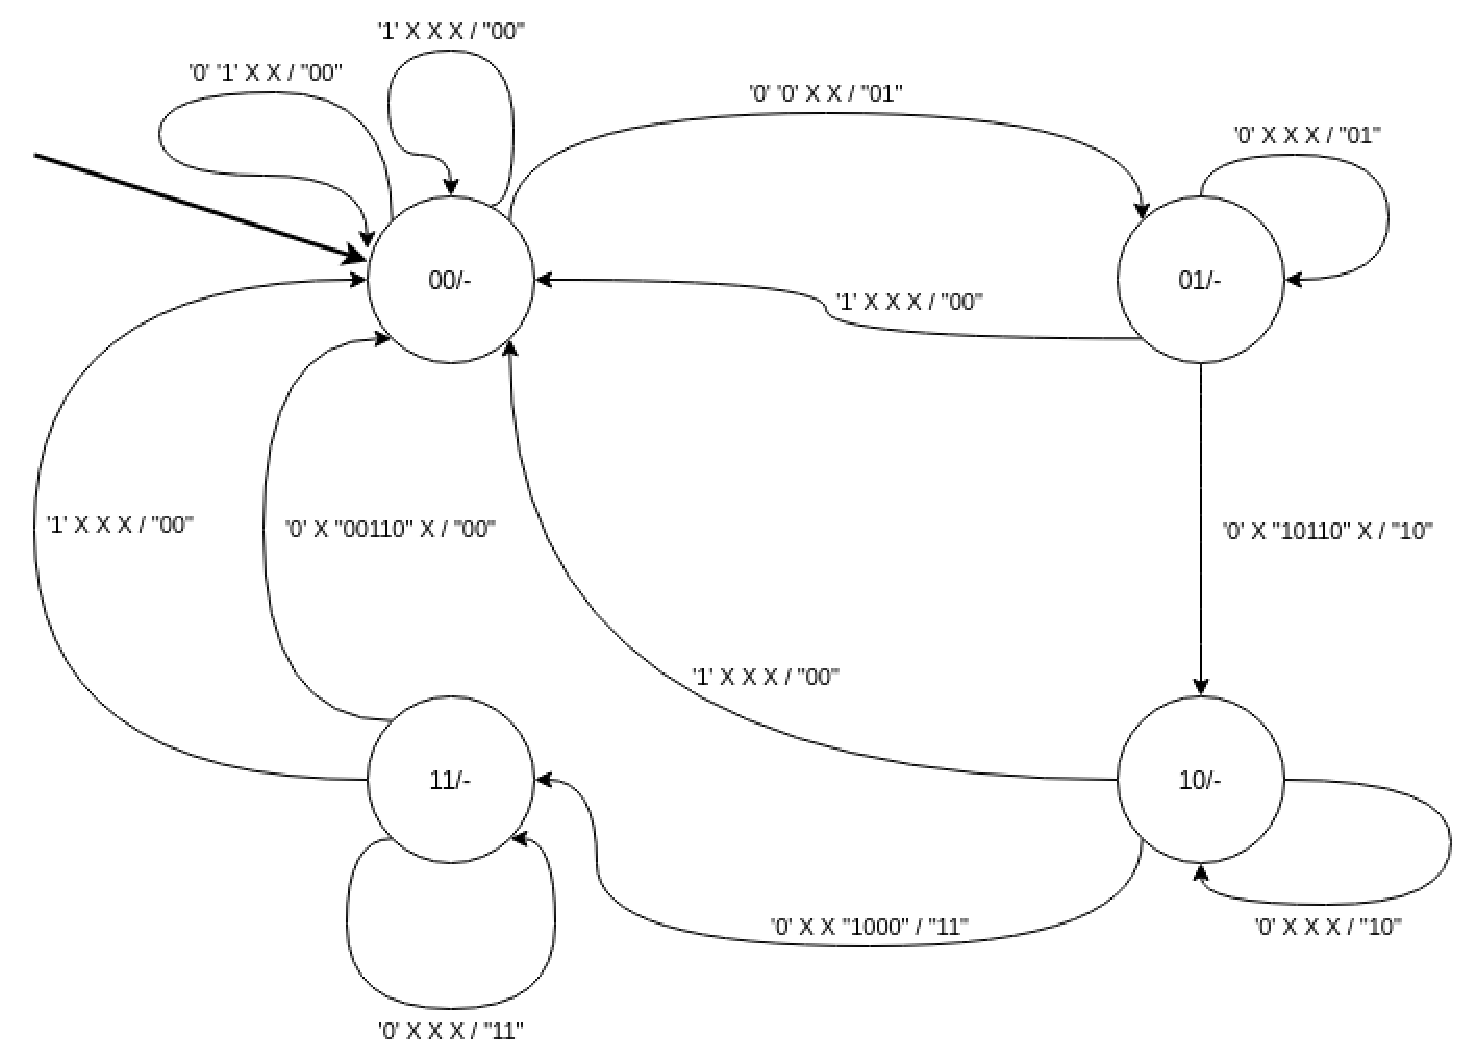
\includegraphics[width=12cm]{src/diag.eps}
  \end{center}
\end{figure}

\subsection*{Popis funkce}
\bigskip
Návrh tohto konečného automatu má len štyri stavy (ako je popísané a zobrazené
vyššie).
\par
Prvým stavom je \textbf{čakanie na start bit} - tu automat začína a nepohne sa 
ďalej, kým nie je \textbf{DIN} nastavený na \emph{log. 0} 
(podľa definície \textbf{UART}). Stav sa potom mení na: \\
\textbf{Čakanie na prvý bit}: medzi nábežnou hranou start bitu a stredom 
prvého bitu je pri nastavení CLK na 16x vyššiu frekvenciu podľa definície UART 
práve \textbf{24} CLK cyklov. Po \textbf{24} nábežných hranách CLK sa stav 
prepne do: \\
\textbf{Prijímanie dát}: V momente prepnutia stavu a potom každú šesťnástu 
nábežnú hranu CLK sa hodnota \textbf{DIN} \uv{skopíruje} na patričný bit 
výstupu. Po prijatí všetkých ôsmich bitov sa prechádza do stavu: \\
\textbf{Koniec}, počas ktorého sa čaká na koniec stop bitu a zároveň sa práve
počas tohto stavu na jeden CLK cyklus nastaví \textbf{DOUT\_VLD} na \emph{log. 1}.
\par
Kedykoľvek v prípade, že je vstup \textbf{RST} nastavený na \emph{log. 1} sa
automat vracia do stavu \uv{čakanie na start bit} ("00").

\newpage


\begin{landscape}
\section*{Snímek obrazovky ze simulací}
\bigskip

\begin{figure}[h]
  \begin{center}
    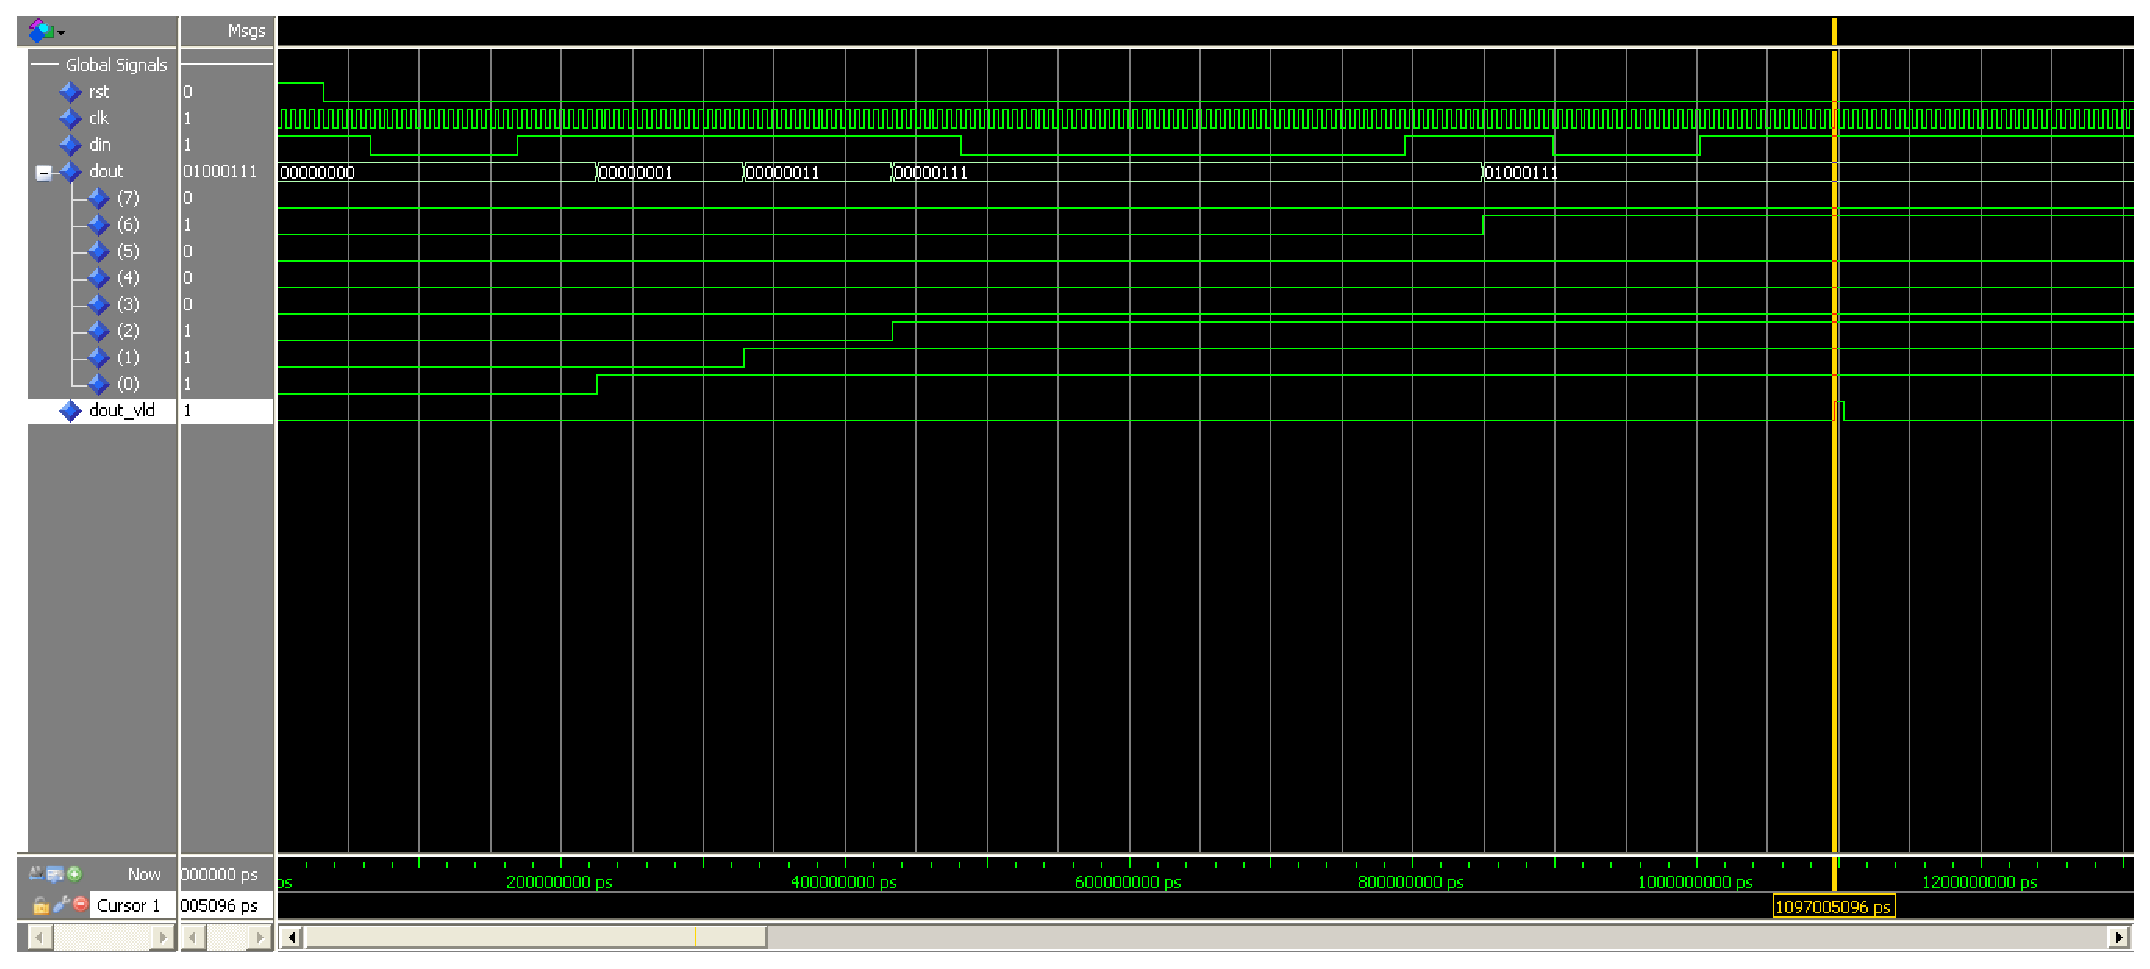
\includegraphics[width=24cm]{src/sim_screenshot.eps}
  \end{center}
\end{figure}
\end{landscape}

\end{document}
